\documentclass[twoside,pl,final]{labman}

\usepackage{graphicx}
\usepackage{float}
\usepackage{url}
\usepackage{listings}
\usepackage[caption=false]{subfig}
\usepackage{placeins}

\graphicspath{ {fig/} }

\subject{Projektowanie układów analogowych dla systemów VLSI}
\title{Lustra prądowe i układ polaryzacji}
\author{mgr inż. Jakub Kopański}

\begin{document}
\maketitle
\tableofcontents
\clearpage
\listoffigures
\clearpage
\listoftables
\clearpage

\chapter{Wstęp}
\label{intro}
Najważniejszym zagadnieniem przy projektowaniu
analogowych układów scalonych jest polaryzacja tranzystorów.
Wybór i zapewnienie odpowiedniego punktu pracy
ma wpływ na szybkość działania układu,
dopasowanie elementów, zakres pracy,
odporność na zakłócenia zasilania i masy
oraz na moc zużywaną przez układ.

W analogowych układach scalonych,
ze względu na łatwość dopasowania elementów,
do polaryzacji tranzystorów wykorzystuję się źródła/lustra prądowe.

W niniejszym ćwiczeniu studenci zapoznają się
z projektowaniem luster prądowych.
Zdobyta wiedza posłuży im do zaprojektowania układu polaryzacji,
który zostanie wykorzystany przy kolejnym ćwiczeniu.

\chapter{Lustra prądowe}
\label{mirror}

\section{Podstawowe lustro prądowe}
\label{mirror:basic}
\begin{figure}[!htbp]
  \centering
  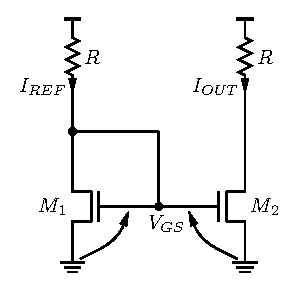
\includegraphics[width=0.4\textwidth]{basic}
  \caption{Podstawowe lustro prądowe}
  \label{fig:basic}
\end{figure}

Podstawowe lustro prądowe,
wykonane z tranzystorów typu~\emph{N},
pokazano na~\fig{fig:basic}
%Przyjmijmy, że oba tranzystory mają takie same wymiary.
Z topologi układu wynika, że~$V_{GS1} = V_{DS1} = V_{GS2}$.
Pomijając wpływ modulacji długości kanału (parametr~$\lambda$),
dzięki równości napięć bramka - źródło obu tranzystorów spodziewamy się,
że oba tranzystory będą miały jednakowy prąd drenu.
Jeżeli oba rezystory mają taką samą wartość rezystancji,
potencjały drenu obu tranzystorów są takie same.
Dopasowując wymiary, napięcia~$V_{GS}$ i prądy drenu~$I_D$ obu tranzystorów,
możemy być pewni, że napięcia dren - źródło obu tranzystorów są jednakowe
($V_{GS1} = V_{DS1} = V_{GS2} = V_{DS2}$).

\begin{figure}[!htbp]
  \centering
  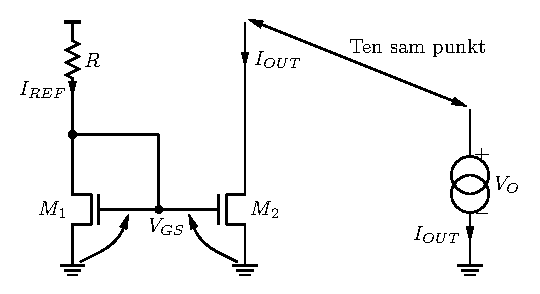
\includegraphics[width=0.7\textwidth]{equiv}
  \caption{Lustro prądowe i schemat zastępczy}
  \label{fig:basic:equiv}
\end{figure}

Na~\fig{fig:basic:equiv} zaprezentowano jak intuicyjne można
myśleć o \emph{wyjściu} lustra prądowego.
W przybliżeniu wyjście lustra prądowego można traktować
jak najprostsze źródło prądowe.
Napięcie na wyjściu lustra prądowego oznaczono~$V_O$.

Założenie, że prądy drenu zależą tylko od panięcia~$V_{GS}$
pomaga zrozumieć działanie lustra prądowego,
ale jest zbyt dużym uproszczeniem.
Dokładniejszą analizę przeprowadzimy już z uwzględnieniem wpływu
modulacji długości kanału.
Prąd płynący w gałęzi referencyjnej lustra jest równy:
\begin{equation}
  I_{REF} = I_{D1} = \frac{K_n}{2} \cdot \frac{W_1}{L_1} \cdot
    (V_{GS1} - V_{TH}) ^ 2 (1 + \lambda V_{DS1}),
  \label{eqn:basic:iref}
\end{equation}
natomiast prąd płynący w gałęzi wyjściowej jest równy:
\begin{equation}
  I_O = I_{D2} = \frac{K_n}{2} \cdot \frac{W_2}{L_2} \cdot
    (V_{GS2} - V_{TH}) ^ 2 (1 + \lambda V_O).
  \label{eqn:basic:iout}
\end{equation}
Jak zostało zauważone we wstępie:~$V_{GS1} = V_{GS2}$,
dzięki temu stosunek prądów drenu tranzystorów ma postać:
\begin{equation}
  \frac{I_O}{I_{REF}} =
  \frac{\frac{K_n}{2} \cdot \frac{W_2}{L_2} \cdot (V_{GS} - V_{TH}) ^ 2 (1 + \lambda V_O)}
  {\frac{K_n}{2} \cdot \frac{W_1}{L_1} \cdot (V_{GS} - V_{TH}) ^ 2 (1 + \lambda V_{DS1})} =
  \frac{W_2 / L_2}{W_1 / L_1}
    \cdot \frac{1 + \lambda V_{O}}{1 + \lambda V_{DS1}}
  \label{eqn:basic:iratio}
\end{equation}

W celu narysowania poprawnej topografii lustra prądowego
długości kanałów tranzystorów muszą być takie same.
Pomijając na razie wpływ modulacji długości kanału,
możemy uprościć~\eqn{eqn:basic:iratio} do postaci:
\begin{equation}
  \frac{I_O}{I_{REF}} = \frac{W_2}{W_1}
  \label{eqn:basic:wratio}
\end{equation}
Poprzez proste skalowanie szerokości kanału,
możemy zmieniać prąd wyjściowy lustra.
Przykładowe zastosowanie pokazano na~\fig{fig:basic:scale}

\begin{figure}[!htbp]
  \centering
  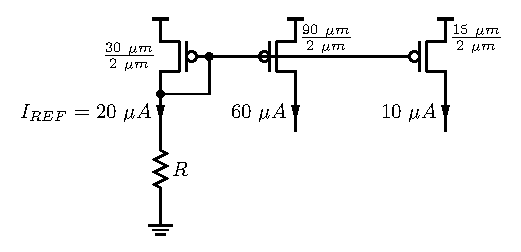
\includegraphics[width=0.6\textwidth]{scale}
  \caption{Skalowanie prądu luster}
  \label{fig:basic:scale}
\end{figure}

\subsection{Dopasowywanie prądów}
\label{matching}
Podstawowym problemem przy projektowaniu lustra prądowego
jest zapewnienie równości prądów referencyjnego~$I_{REF}$
oraz wyjściowego~$I_O$.
W następnych sekcjach zbadamy jak różnice parametrów
wpływają na różnice prądów.

\subsubsection{Różnica napięć progowych}
\label{mirror:matching:vth}
W punkcie~\ref{mirror:basic} powiedzieliśmy,
że w pierwszym przybliżeniu, równość prądów $I_{REF}$ oraz $I_O$
wynika z równości napięć $V_{GS}$ lustra prądowego.
Do dobrego dopasowania prądów, niezbędne jest dopasowanie
napięć progowych obu tranzystorów lustra prądowego.
Chcąc zbadać wpływ różnicy napięć progowych przyjmujemy, źe:
\begin{eqnarray}
  V_{TH1} &= V_{TH} - \frac{\Delta V_{TH}}{2}, \nonumber \\
  V_{TH2} &= V_{TH} + \frac{\Delta V_{TH}}{2}.
  \label{eqn:matching:vth}
\end{eqnarray}
Obliczając stosunek prądów lustra z
wykorzystaniem~\eqn{eqn:matching:vth}, otrzymujemy:
\begin{equation}
  \frac{I_O}{I_{REF}} = \frac{\frac{K_n}{2} \frac{W}{L} (V_{GS} - V_{TH} - \frac{\Delta V_{TH}}{2})^2}
    {\frac{K_n}{2} \frac{W}{L} (V_{GS} - V_{TH} + \frac{\Delta V_{TH}}{2})^2} =
    \frac{\big[1 - \frac{\Delta V_{TH}}{2 (V_{GS} - V_{TH})}\big]^2}
    {\big[1 - \frac{\Delta V_{TH}}{2 (V_{GS} - V_{TH})}\big]^2}
  \label{eqn:matching:vth:ratio}
\end{equation}
Podnosząc wyrażenia do kwadratu, a następnie zaokrąglając poprzez pominięcie
wyrażeń w wyższych potęgach, stosunek prądu wynosi w przybliżeniu:
\begin{equation}
  \frac{I_O}{I_{REF}} \approx 1 \frac{2 \Delta V_{TH}}{V_{GS} - V_{TH}} =
    1 - \frac{2 \Delta V_{TH}}{V_{DSsat}}
  \label{eqn:matching:vth:approx}
\end{equation}
Wyrażenie~\eqn{eqn:matching:vth:approx} dobrze ilustruje jakość
dopasowania prądów w zależności od napięcia progowego~$V_{TH}$.
Im większa różnica napięć progowych, tym większa różnica prądów:
referencyjnego i wyjściowego prądu lustra.
Im mniejsze napięcie bramka - źródło tranzystorów lustra prądowego,
tym większy wpływ różnicy napięć progowych.
Aby zminimalizować wpływ różnicy napięć progowych należy pracować przy
wyższym napięciu~$V_{GS}$ pamiętając, że kosztem takiego zabiegu będzie
mniejszy zakres napięcia wyjściowego tranzystora~$V_{DS}$,
dla którego tranzystor pozostaje w nasyceniu.

\subsubsection{Różnica transkonduktancji}
\label{baisc:matching:kp}
Podobna analiza może być przeprowadzona dla różnicy parametru~$K_n$ tranzystora.
Jeżeli przyjmiemy, że:
\begin{align}
  K_{n1} &= K_n - \frac{\Delta K_n}{2}, \nonumber \\
  K_{n2} &= K_n + \frac{\Delta K_n}{2},
\end{align}
to wówczas zakładając, że pozostałe parametry tranzystorów lustra
są takie same, stosunek prądów wynosi:
\begin{equation}
  \frac{I_O}{I_{REF}} = \frac{K_n + \frac{\Delta K_n}{2}}
    {K_n - \frac{\Delta K_n}{2}} \approx
    1 + \frac{\Delta K_n}{K_n}
  \label{eqn:matching:kp}
\end{equation}
Parametr~$K_n$ jest parametrem technologicznym,
który zależy od procesu wytwarzania układów scalonych.
Mogłoby się wydawać, że wraz ze skalowaniem procesu różnice w~$K_n$
tranzystorów spowodowane różnicami w tlenku bramkowym oraz
różnicami ruchliwości powinny być mniejsze.
Jednak mniejsze wymiary tranzystorów powodują również,
że jeżeli wystąpi defekt to jest on uśredniany
po mniejszej powierzchni przyrządu.

\subsubsection{Różnica napięć $V_{DS}$}
\label{matching:vds}

\begin{figure}[!htbp]
  \centering
  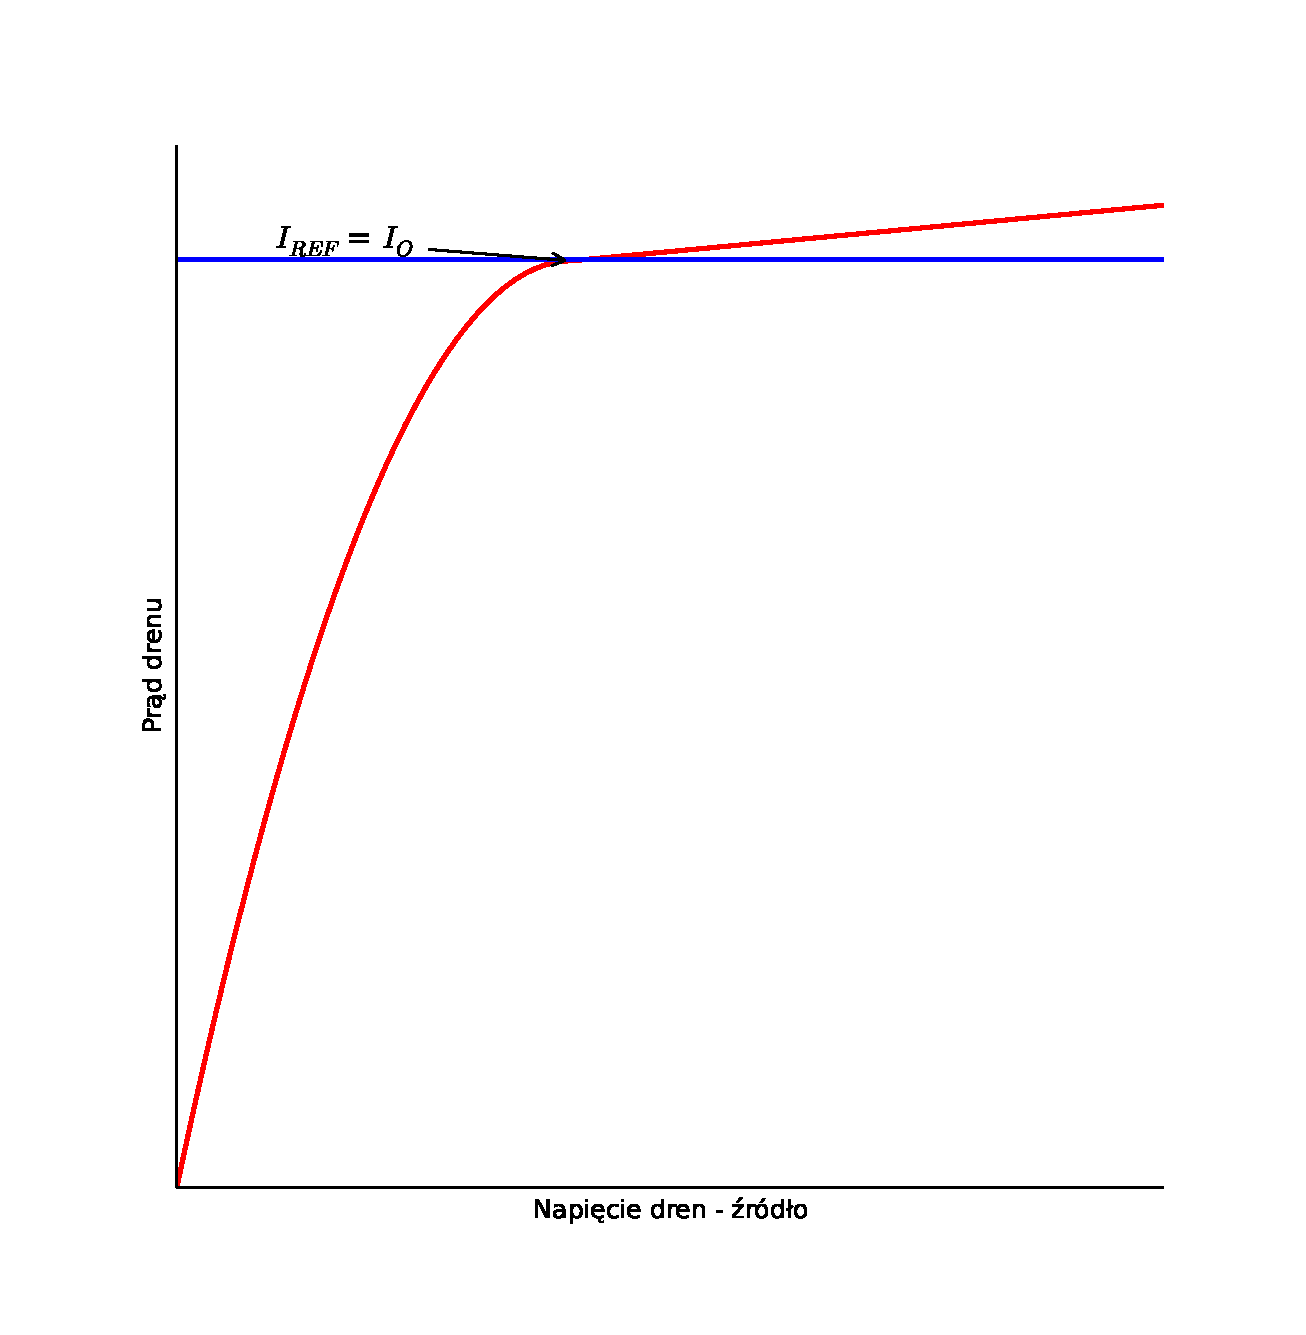
\includegraphics[width=0.5\textwidth]{matching_vds}
  \caption{Zależność prądu od napięcia~$V_{DS}$.}
  \label{fig:matching:vds}
\end{figure}

Efektem który bardzo silnie wpływa na dopasowanie prądów lustra jest
różnica napięcia dren - źródło tranzystorów.
Rys~\ref{fig:matching:vds} przedstawia wartości prądów~$I_{REF}$
oraz~$I_O$ w zależności od napięcia wyjściowego~$V_O$
lustra ze schematu na~\fig{fig:basic:equiv}.
Jak można zauważyć prądy są jednakowe tylko dla jednej,
konkretnej wartości napięcia~$V_O$,
równej napięciu~$V_{DS}$ tranzystora referencyjnego~$M_1$.
Biorąc pod uwagę różnice napięć~$V_{DS}$ tranzystorów
oraz parametr~$\lambda$, stosunek prądów lustra można zapisać jako:
\begin{equation}
  \frac{I_O}{I_{REF}} = \frac{1 + \lambda_2 V_{O}}{1 + \lambda_1 V_{DS}}
  \label{eqn:matching:vds}
\end{equation}

W tym miejscu warto policzyć stosunek~\eqn{eqn:matching:vds}
dla konkretnych realnych wartości, (które autor niniejszej instrukcji uzyskał
wykonując pierwsze ćwiczenie).
Zakładając, że~$\lambda_1 = \lambda_2 = 0,36 \frac{1}{V}$ oraz~$V_{DS} = 192~mV$
i $V_O = V_{DS} + 0.6~V = 792~mV$ otrzymujemy:
\begin{equation}
  \frac{I_O}{I_{REF}} = \frac{1 + 0,36 \times 0,792~V}
    {1 + 0,36 \times 0,192~V} \approx 1,20
  \label{eqn:matching:result}
\end{equation}
co oznacza \emph{niedopasowanie prądów lustra aż o 20~\%}.
Jak widać równość napięć dren - źródło tranzystorów tworzących zwierciadło
prądowe ma krytyczne znaczenie dla równości prądów,
dlatego w kolejnych rozdziałach przedstawimy sposoby
na ograniczenie wpływu różnicy napięć~$V_{DS}$.

\section{Kaskodowe lustro prądowe}
\label{cascode}
Rozwiązaniem problemu różnych napięć dren - źródło tranzystorów
tworzących lustro prądowe jest kaskodowe lustro prądowe.

\subsection{Prosta kaskoda}
\label{cascode:simple}

\begin{figure}[!htbp]
  \centering
  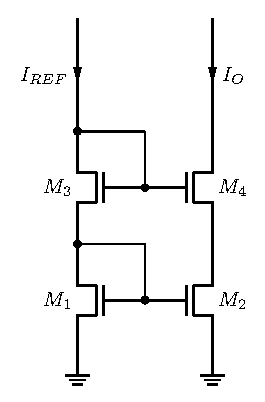
\includegraphics[width=0.3\textwidth]{cascode_simple}
  \caption{Kaskodowe lustro prądowe.}
  \label{fig:cascode:simple}
\end{figure}

Najprostsze kaskodowe lustro prądowe zaprezentowano na~\fig{fig:cascode:simple}
Prąd w gałęzi wyjściowej jest wymuszany przez tranzystor~$M_2$.
Napięcie na bramce tego tranzystora jest ustalane
przez tranzystor~$M_1$ w połączeniu diodowym.
Napięcie~$V_{DS}$ tranzystora~$M_2$ jest ustalane przez tranzystor~$M_4$,
jest ono równe napięciu na bramce tranzystora~$M_4$,
pomniejszone o jego napięcie~$V_{GS}$.
Napięcia w poszczególnych węzłach układu
zaznaczono na~\fig{fig:cascode:simple:node}

\begin{figure}[!htbp]
  \centering
  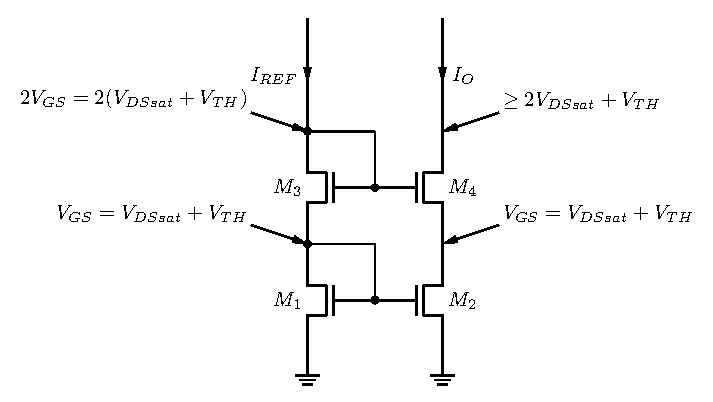
\includegraphics[width=0.9\textwidth]{cascode_simple_node}
  \caption{Wartości napięć w kaskodowym lustrze prądowym.}
  \label{fig:cascode:simple:node}
\end{figure}

\subsection{Kaskoda o obniżonym napięciu wyjściowym}
\label{cascode:wideswing}

\begin{figure}[!htbp]
  \centering
  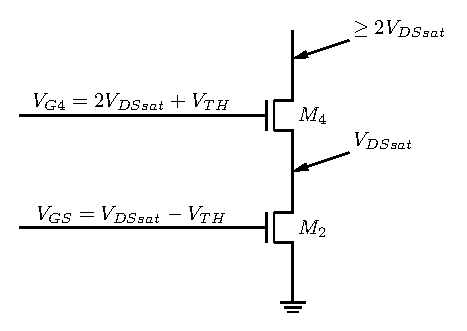
\includegraphics[width=0.4\textwidth]{cascode_wideswing}
  \caption{Idea niskonapięciowej kaskody.}
  \label{fig:cascode:wideswing:idea}
\end{figure}

Problemem kaskody opisanej w ostatnim punkcie jest wysoka wartość minimalnego
napięcia wyjściowego takiego lustra prądowego,
równa: $2 \times V_{DSsat} + V_{TH}$.
Wyjściem lustra jest szeregowe połączenie 2 tranzystorów.
Minimalnym napięciem jakie powinno być potrzebne
aby tranzystory pozostały w nasyceniu jest: $2 \times V_{DSsat}$.
Rys~\ref{fig:cascode:wideswing:idea} przedstawia
wymagane napięcia dla kaskody o obniżonym napięciu wyjściowym.

\subsubsection{Generowanie napięcia polaryzacji tranzystora kaskodującego}
\label{cascode:wideswing:mws}

\begin{figure}[!htbp]
  \centering
  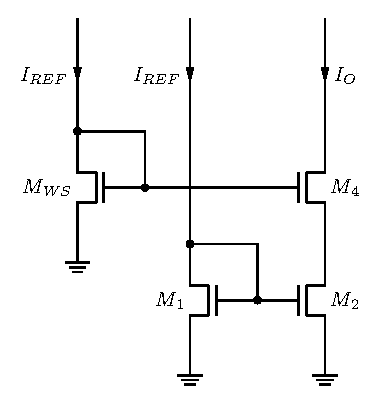
\includegraphics[width=0.5\textwidth]{cascode_gen}
  \caption{Generowanie dodatkowego napięcia dla kaskody.}
  \label{fig:cascode:wideswing:gen}
\end{figure}

Aby wygenerować napięcie~$2 \times V_{DSsat} + V_{TH}$ potrzebne
dla bramki tranzystora~$M_4$, należy rozdzielić generowanie napięć dla bramek
tranzystorów~$M_4$ i~$M_2$ na oddzielne gałęzie.
Rozwiązanie zostało zaprezentowane na~\fig{fig:cascode:wideswing:gen}
W celu uzyskania odpowiedniego napięcia na bramce tranzystora~$M_4$
możemy zmienić wymiary ($W$~i~$L$) tranzystora~$M_{WS}$.
Napięcie $V_{GS}$ tranzystora $M_{WS}$ musi być równe wymaganemu
napięciu ($2 \times V_{DSsat} + V_{TH}$) na bramce tranzystora~$M_4$.
Stąd mamy:
\begin{align}
  I_{REF} &= \frac{K_n}{2} \frac{W_{M_{WS}}}{L_{M_{WS}}}
    \big(2 ( V_{GS} - V_{TH}) + V_{TH} - V_{TH} \big)^2, \nonumber \\
  I_{REF} &= \frac{K_n}{2} \frac{W_{M_{WS}}}{L_{M_{WS}}}
    4 ( V_{GS} - V_{TH} )^2. \nonumber \\
\end{align}
Przyrównując prądy płynące przez tranzystory $M_1$ i $M_{WS}$ otrzymujemy:
\begin{equation}
  \frac{W}{L} = \frac{W_{M_{WS}}}{L_{M_{WS}}} \times 4,
\end{equation}
lub gdy przyjmiemy takie same szerokości tranzystorów:
\begin{equation}
  L_{M_{WS}} = 4 \times L.
\end{equation}
Aby uzyskać napięcie niezbędne do polaryzacji bramki tranzystora~$M_4$
(a przez co wymuszenia odpowiedniego napięcia na drenie tranzystora~$M_2$)
należy użyć tranzystora o~$4$ razy dłuższym kanale.

Ze względu na lepsze dopasowanie tranzystorów podczas
rysowania topografii układu,
tranzystor~$M_{WS}$ realizuje się jako szeregowe połączenie tranzystorów,
o takiej samej długości kanału jak pozostałe tranzystory lustra.
Sposób realizacji widać na~\fig{fig:cascode:wideswing:mws}
Długość kanału tranzystora~$M_{WS}$ równa czterem długościom
kanału typowego tranzystora spowoduje,
że napięcie~$V_{DS}$ tranzystora~$M_2$ będzie na granicy nasycenia.
Ze względu na rozrzuty produkcyjne czy wahania napięcia zasilania
może zdarzyć się, że napięcie na drenie~$M_2$ obniży się i tranzystor
\emph{wypadnie} z obszaru nasycenia.
Dlatego należy zwiększyć trochę wartość napięcia na bramce~$M_4$,
poprzez uczynienie tranzystora~$M_{WS}$ dłuższym.
Typowo jego długość dobiera się eksperymentalnie,
tak aby $M_2$ pozostał w nasyceniu, z pewnym zapasem.

\begin{figure}[!htbp]
  \centering
  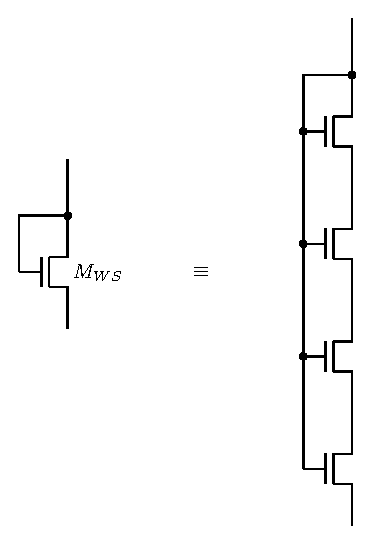
\includegraphics[width=0.3\textwidth]{cascode_mws}
  \caption{Realizacja tranzystora $M_{WS}$.}
  \label{fig:cascode:wideswing:mws}
\end{figure}

\subsubsection{Wyrównanie napięć $V_{DS}$}
\label{cascode:wideswing:vds}

Uważny czytelnik może zauważyć, że tranzystory~$M_1$~i~$M_2$
mają różne napięcia~$V_{DS}$.
Jak zostało napisane w sekcji~\ref{matching:vds}
równość napięć dren - źródło tranzystorów jest krytycznym czynnikiem
wpływającym na równość prądów drenu.
Rozwiązanie tego problemu przedstawiono na~\fig{fig:cascode:wideswing:vds}
Jest nim dodanie kolejnego tranzystora, który podobnie jak~$M_4$,
wymusi odpowiednie napięcie~$V_{DS}$ tranzystora referencyjnego~$M_1$.

\begin{figure}[!htbp]
  \centering
  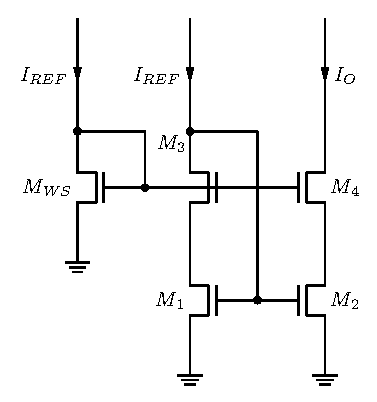
\includegraphics[width=0.5\textwidth]{cascode_vds}
  \caption{Wyrównanie napięć $V_{DS}$ tranzystorów lustra.}
  \label{fig:cascode:wideswing:vds}
\end{figure}

\chapter{Układ polaryzacji}
\label{bias}

\begin{figure}[!htbp]
  \centering
  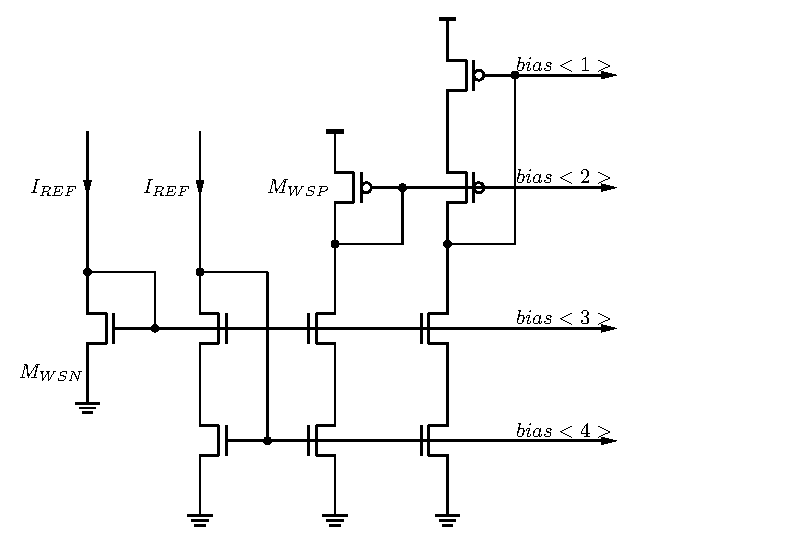
\includegraphics[width=0.8\textwidth]{bias}
  \caption{Układ polaryzacji projektowany na zajęciach.}
  \label{fig:bias}
\end{figure}

Przedstawione w poprzednim rozdziale kaskodowe lustro prądowe o zwiększonym
zakresie napięcia wyjściowego jest podstawą bloku polaryzacji,
jaki należy zaprojektować podczas laboratorium.
Przedstawiony schemat jest uproszczony aby skupić się na tym co jest istotne.
Blok generuje napięcia~$bias~<~1~:~4~>$,
które można wykorzystać do zrobienia źródeł prądowych o dowolnej wartości.
Układ to nic innego, jak połączone kaskodowe
lustra prądowe z tranzystorów typu $N$~i~$P$.

\chapter{Projekt bloku polaryzacji}
\label{work}

Na zajęciach należy zmodyfikować blok~\emph{bias\_hs\_10u}
z biblioteki \emph{LIB2}.
Dla projektowanego bloku przygotowane zostało
środowisko testowe~\emph{bias\_sim}.
Najważniejsze mierzone parametry zebrane
zostały w~\tab{tab:work:measure}.

Celem ćwiczenia jest takie zaprojektowanie układu polaryzacji,
aby możliwe było proste zrobienie nowych źródeł prądowych,
poprzez wykorzystanie napięć~$bias~<~1~:~4~>$.
Prąd wyjściowy źródła~$i_bias$ powinien mieć wartość
równą prądowi referencyjnemu (w tym przypadku $10~\mu{}A$),
z dokładnością~$\pm~5~\%$.

Następnie należy policzyć teoretyczną wartość rezystancji wyjściowej
źródeł (kaskodowego i zwykłego) i porównać ją
z wynikami otrzymanymi z symulacji elektrycznej.
W odróżnieniu od pierwszego ćwiczenia,
należy przeprowadzić symulacje w narożnikach procesu
\eng{process corners} i podczas rozrzutów produkcyjnych z
wykorzystaniem analizy \emph{Monte Carlo}.

\begin{table}[htbp]
  \centering
  \caption{Mierzone parametry luster prądowych}
  \label{tab:work:measure}
  \begin{tabular}{l p{0.7\textwidth}}
    \hline \hline
    Nazwa & Opis \\
    \hline
    $i\_bias$ & Prąd wyjściowy lustra prądowego \\
    $ron@vds$ & Rezystancja wyjściowa zwykłego lustra prądowego przy napięciu wyjściowym równym $vdsn$ \\
    $rop@vds$ & Rezystancja wyjściowa zwykłego lustra prądowego przy napięciu wyjściowym równym $vdsp$ \\
    $ron\_casc@vds$ & Rezystancja wyjściowa kaskodowego lustra prądowego przy napięciu wyjściowym równym $vdsn\_casc$ \\
    $rop\_casc@vds$ & Rezystancja wyjściowa kaskodowego lustra prądowego przy napięciu wyjściowym równym $vdsp\_casc$ \\
    $vdsn$ & Wartość napięcia wyjściowego zwykłego lustra prądowego, dla którego rezystancja wyjściowa rośnie najszybciej \\
    $vdsp$ & Wartość napięcia wyjściowego zwykłego lustra prądowego, dla którego rezystancja wyjściowa rośnie najszybciej \\
    $vdsn\_casc$ & Wartość napięcia wyjściowego kaskodowego lustra prądowego, dla którego rezystancja wyjściowa rośnie najszybciej \\
    $vdsp\_casc$ & Wartość napięcia wyjściowego kaskodowego lustra prądowego, dla którego rezystancja wyjściowa rośnie najszybciej \\
    \hline \hline
  \end{tabular}
\end{table}

\section{Symulacja w narożnikach procesu}
\label{work:corners}

\begin{figure}[!htbp]
  \centering
  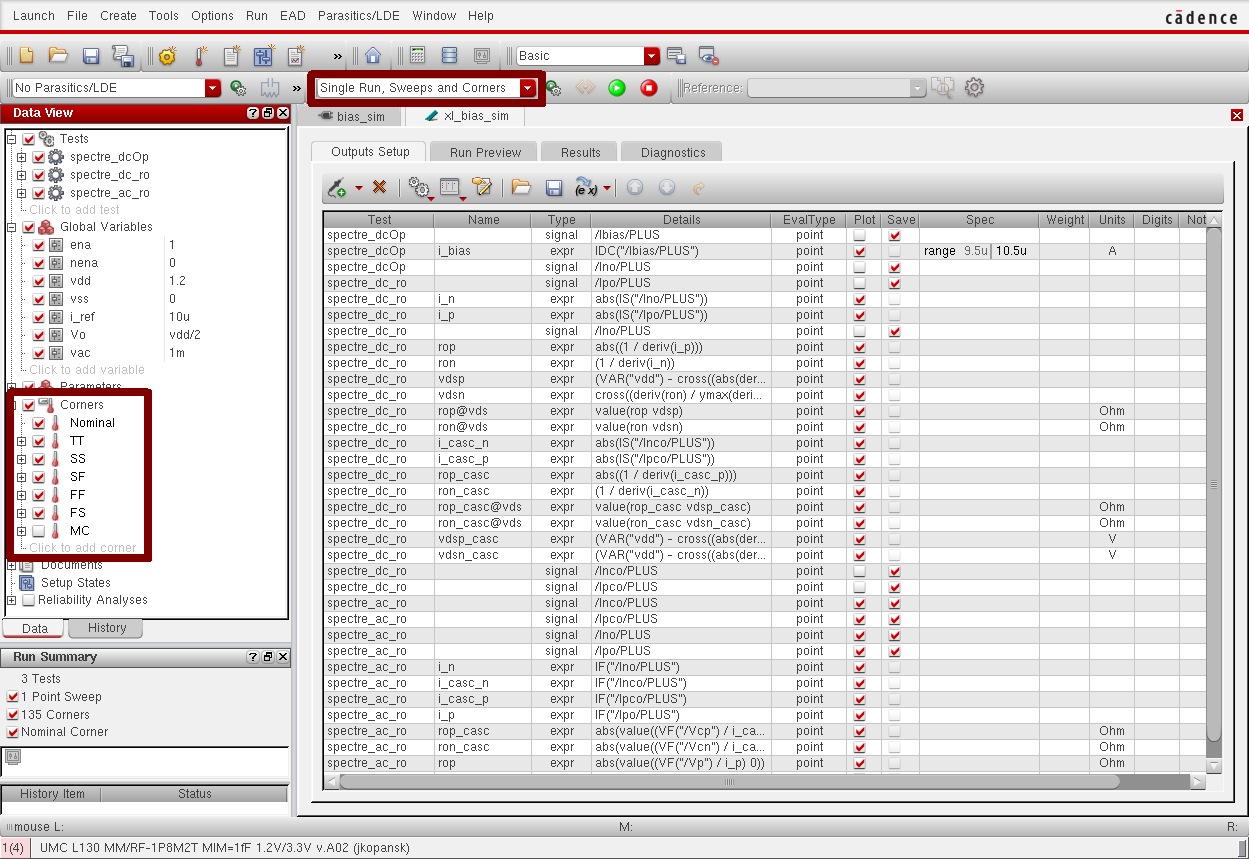
\includegraphics[width=0.9\textwidth]{corners}
  \caption{Konfiguracja symulacji narożników procesu.}
  \label{fig:work:corners}
\end{figure}

W celu uruchomienia symulacji \emph{process corners} należy zaznaczyć
opcje \emph{corners} w panelu po lewej stronie okna \emph{ADE (G)XL}
a następnie wybrać, które skrajne przypadki chcemy symulować.
Litery~\emph{T}, \emph{F}, \emph{S} oznaczają przypadki:
\emph{Typical}, \emph{Fast} i \emph{Slow} tranzystorów \emph{MOS}.
Pierwsza litera w nazwie narożnika procesu odnosi się do
tranzystora typu~\emph{N}, druga zaś typu~\emph{P}.
Opcja~\emph{MC} dotyczy symulacji \emph{Monte Carlo} i w przypadku narożników
procesów \emph{nie może} być zaznaczona.
Prawidłowa konfiguracja przedstawiona jest na~\fig{fig:work:corners}

\section{Analiza Monte Carlo}
\label{work:montecarlo}

\begin{figure}[!htbp]
  \centering
  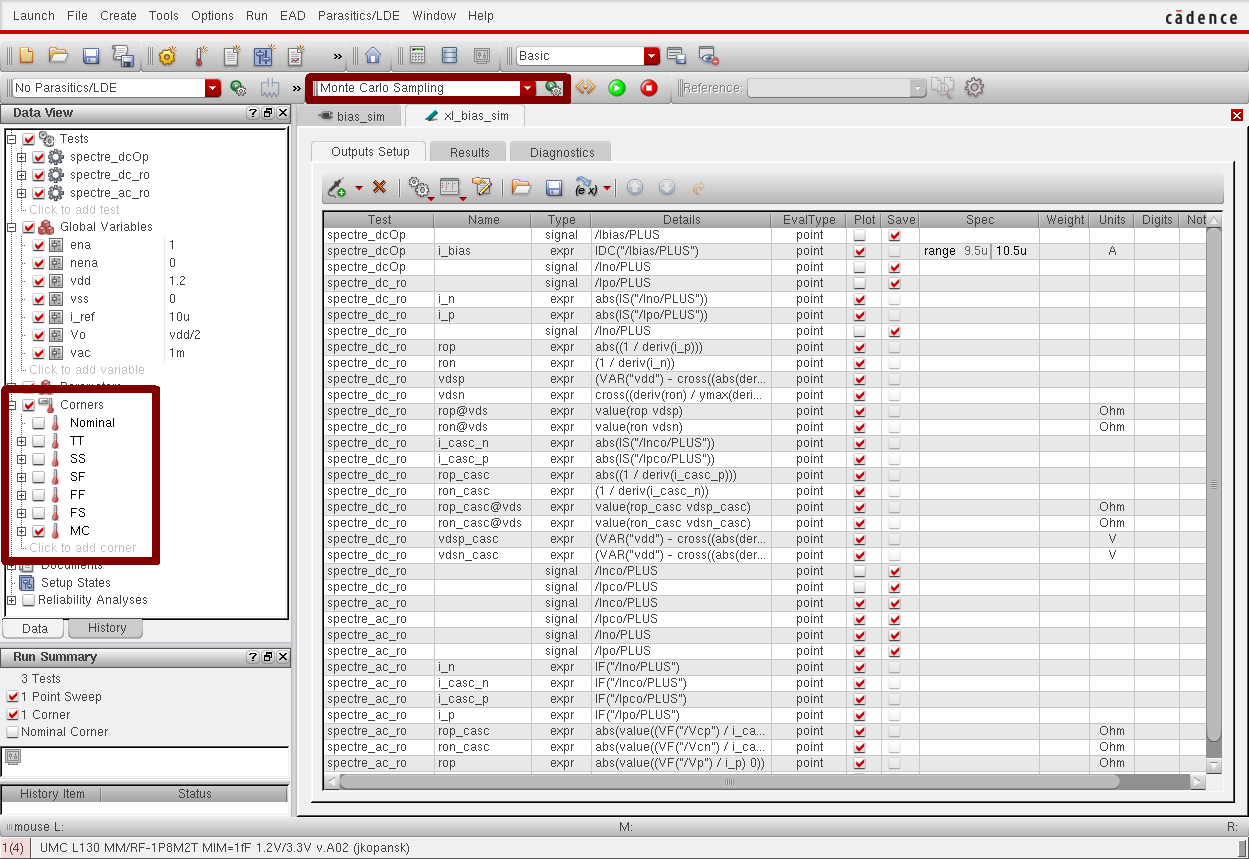
\includegraphics[width=0.9\textwidth]{mc}
  \caption{Konfiguracja analizy Monte Carlo.}
  \label{fig:work:mc}
\end{figure}

Aby wykonać analizę \emph{Monte Carlo} należy wybrać specjalny przypadek
analizy narożników procesu, nazwany~\emph{MC}.
\emph{Musi} to być jedyny zaznaczony skrajny przypadek.
Należy także przed uruchomieniem symulacji wybrać jej rodzaj z rozwijanej listy
na pasku narzędzi.
Ustawienia pokazano na~\fig{fig:work:mc}
Symulacje \emph{Monte Carlo} należy jeszcze skonfigurować,
a dokładnie podać ilość niezależnych symulacji z różnymi wartościami
parametrów poddanych rozrzutom.
Okno konfiguracji analizy wywołuje się poprzez kliknięcie ikonki
obok listy wyboru rodzaju analizy,
ikonę zaznaczono razem z listą również na~\fig{fig:work:mc}
Samo okno konfiguracji wraz z zaznaczonym polem do uzupełnienia
przedstawia~\fig{fig:work:mc:setup}

\begin{figure}[!htbp]
  \centering
  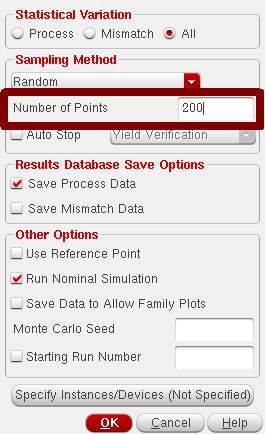
\includegraphics[width=0.3\textwidth]{mc_setup}
  \caption{Opcje analizy Monte Carlo.}
  \label{fig:work:mc:setup}
\end{figure}

\subsection{Równoległe uruchamianie symulacji}
\label{work:parallel}

\begin{figure}[!htbp]
  \centering
  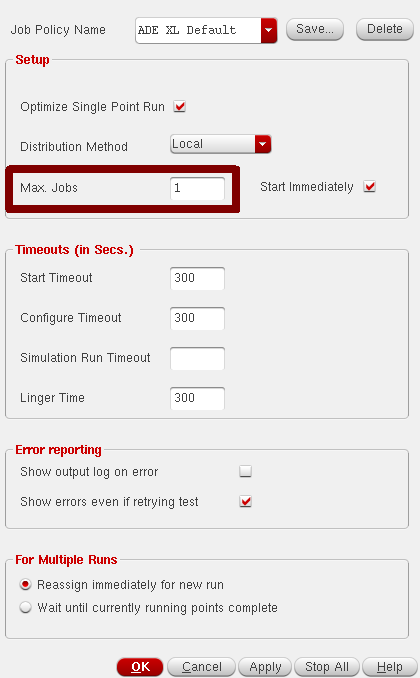
\includegraphics[width=0.3\textwidth]{jobs_setup}
  \caption{Opcje konfiguracji procesów.}
  \label{fig:work:jobs:setup}
\end{figure}

Zarówno analiza \emph{process corners} jak i \emph{Monte Carlo}
wykonuje wiele niezależnych symulacji,
dlatego idealnie nadaje się do zrównoleglenia poprzez uruchomienie jej
w wielu procesach.
Opcje dotyczące ilości wykorzystywanych wątków znajdują się w menu:
\emph{Options}~$\rightarrow$~\emph{Job Setup...}
i zaprezentowano je na~\fig{fig:work:jobs:setup}

\bibliographystyle{IEEEtran}
\bibliography{IEEEabrv,bibliography}

\end{document}
